%!TEX root = MagicSquare.tex
We now apply the results of the previous section to conclude robustness for a specific family of games.
We must both understand the representation theory of their abstract solution groups and the combinatorics of the presentations for those groups. Even though our general robust self-testing theorem holds for LCS games mod $d$, we are currently only aware of applications of it to examples of LCS games mod $2$. In this section, we show applications of our theorem to the magic square and magic pentagram games mod $2$, and to certain parallel versions of these games.

\subsection{The qudit pauli group}
In this subsection, we formally introduce the Pauli group. We state definitions and prove properties for the Pauli group mod $d$. However, we will later only utilize such properties for the Pauli group mod $2$. As mentioned earlier, a manuscript by Joel Wallman, to appear shortly after this one, shows that there does not exist any pseudotelepathy LCS game mod $d$, for $d\neq 2$, whose ideal strategy consists of products of Pauli operators.
\begin{definition}\label{definition:n-qudit-pauli-group}
	The $n$-qudit Pauli group of local dimension $d$ is denoted $\m P_d^{\otimes n} := \braket{S:R}_{\Z_d}$ and presented with generators and relations
	\begin{align}
		S = \set{x_i,z_i\;i\leq n}
		&&
		R = \set{J\1[x_i,z_i], [x_i,x_j], [z_i,z_j], [x_i,z_j]\;i \neq j \leq n}
	\end{align}
\end{definition}

We aim to show that the Pauli group is suitable for applying the results from Section \ref{sec:self-testing}. 

\begin{definition}
\label{def:representations-pauli-group}
	We now define maps $\tau_l^{(n)}: \m P_d^{\otimes n} \to U(\C^{d})^{\otimes n}$ as 
	\begin{align}
	\tau_l^{(n)}(J) &= \w_d^l I
	,
	\\\tau_l^{(n)}(x_i) &= \underbrace{I\otimes \cdots I}_{i-1} \otimes X^l \otimes \underbrace{I \otimes\cdots \otimes I}_{n-i}
	,
	\\\tau_l^{(n)}(z_i) &= \underbrace{I\otimes \cdots I}_{i-1} \otimes Z \otimes \underbrace{I \otimes\cdots \otimes I}_{n-i}.
	\end{align}
\end{definition}
\begin{lemma}
\label{lemma:representations-pauli-group}
	The $\set{\tau_l^{(n)}\;l\in \Z_d\minus\set0}$ are $d-1$ inequivalent representations of dimension $d^n$. 
\end{lemma}
\begin{proof}
	To see that they are representations, it suffices to check the commutation and anticommutation relations. To see that they are inequivalent, see that their characters differ at $J$, since $\Tr\tau_l^{(n)}(J) = \w_d^ld^n$. 
\end{proof}

\begin{prop}\label{prop:representations-pauli-group}
	$\m P_d^{\otimes n}$ group-tests $\tau_1^{(n)}$ in the sense of Definition \ref{definition:group-test}.
\end{prop}

To prove this, we first establish the following lemma, which will let us count the elements of $\pauli$.

\begin{lemma}
\label{lemma:canonical-form}
	There is a canonical form $\can: \m P_d^{\otimes n} \to \m F(S)$ which sends each element to a string of the form
	\begin{equation}
	 	J^{a_1}\prod_{i=1}^nx_i^{a_{2i}}z_i^{a_{2i+1}}, a_i\in \Z_d.
	 \end{equation}
\end{lemma}
\begin{proof}
	First, we see that each element can be written this way. Start with an arbitrary word representing the element and apply the commutation and anticommutation relations to get the $x_i$ and $z_i$ in order. Finish by commuting all of the $J$s to the front and applying the relations $s^d = 1$ to get all of the exponents to lie in $\Z_d$. 

	Next, we see that different words represent different group elements. Suppose that 
 	\begin{equation}\label{eq:canonical-form}
 		J^{a_1}\prod_{i=1}^nx_i^{a_{2i}}z_i^{a_{2i+1}} = J^{b_1}\prod_{i=1}^nx_i^{b_{2i}}z_i^{b_{2i+1}}.
 	\end{equation}
 	Then by various applications of the (twisted) commutation relations, we have
 	\begin{equation}\label{eq:canonical-form-uniqueness}
 		J^{c_1} = \prod_{i=1}^nx_i^{a_{2i} - b_{2i}}z_i^{a_{2i+1}-b_{2i+1}}
 	\end{equation}
 	for some $c_1 \in \Z_d$. The left hand side is always central, but the right hand side is central only if $a_i = b_i$ for all $i\in [2,2n+1]$. 
 	(Suppose for example that $a_3 - b_3 \neq 0$, so that the power of $z_1$ is nonzero. Then the right hand side fails to commute with $x_1$.) 
 	In this case, we can see that in fact $c_1 = a_1 - b_1$, so equation \eqref{eq:canonical-form-uniqueness} holds only if $J^{c_1} = 1$ in the group. 
 	 But Proposition \ref{lemma:representations-pauli-group} gives us a representation in which $J$ and $1$ are represented by distinct matrices. Therefore, equation \eqref{eq:canonical-form-uniqueness} holds only when $a_i = b_i$ for all $i$.
\end{proof}

Thanks to the canonical form, we can easily compute the size of $\m P_d^{\otimes n}$.
\begin{cor}
	$\m P_d^{\otimes n}$ has $d^{2n+1}$ elements.
\end{cor}
\begin{proof}[Proof of Proposition \ref{prop:representations-pauli-group}]
	We'll check that $\m P_d^{\otimes n}$ has exactly $d-1$ irreducible representations of dimension $d^{n}$, each sending $J$ to a different nontrivial $d\th$ root of unity. All other irreducible representations are $1$-dimensional and send $J$ to $1$. 

	We'll complete the character table of $\pauli$. Now that we know the size of the group, we can check via Fact \ref{fact:irreducibility-criterion} that the representations of Lemma \ref{lemma:representations-pauli-group} are irreducible. 

	Next, we notice that the commutator subgroup $[\m P_d^{\otimes n},\m P_d^{\otimes n}]$ is equal to $\braket J$, the cyclic subgroup generated by $J$. This has order $d$, so by Fact \ref{fact:1-dim-irreps}, there are $d^{2n}$ irreps of dimension $1$ which send $J$ to $1$. Now we add the squares of the dimensions of our irreps and see that they saturate equation \eqref{eq:character-dimension}.
	\begin{equation}
		\abs\pauli = d^{2n+1} = (d-1)\cdot (d^n)^2 + (d^{2n})\cdot(1)^2 = \sum_\s (\dim \s)^2.
	\end{equation}
	Therefore, we've found all irreducible representations of $\pauli$. 
\end{proof}

\begin{lemma}\label{lemma:small-group-pictures-pauli-n}
	Let $\can$ be the canonical form from Lemma \ref{lemma:canonical-form}. Then each equation $\can(x)\can(yx)\1\can(y) = 1$ is witnessed by a $\pauli$-picture in which
	each generator and each relation appears at most $18d^2n$ times.
\end{lemma}
\begin{proof}
	See Figure \ref{fig:small-group-pictures-pauli-n}. Starting from arbitrary $x, y$, we compute $\can(x), \can(y), \can(yx)\1$. Draw a group picture whose boundary is $\can(x)\can(yx)\1\can(y)$ up to $J$ terms. Link each positive term from $\can(x)$ and $\can(y)$ with an appropriate negative term from $\can(yx)\1$. In the case that there are more positive terms than negative terms, link them with each other using a relation of the form $s^d=1$. At each intersection of links, add a vertex with either a commutation relation or an anticommutation relation. This subdivides the links into edges, giving us a valid group picture. Now we compute its size.

	There are $2n$ generators and each generator has multiplicity at most $d$ in each of $\can(x), \can(xy)\1, \can(y)$. Therefore, we draw at most $3d\cdot 2n$ links in the above drawing process. Each link intersects each other link at most once, so each link is subdivided into at most $6dn$ edges. Each generator labels at most $3d$ links, so there are at most $18d^2n$ edges with a given label. We must also count the uses of the generators. Recall that each relation involves only two generators. Therefore, each relation is used at most $(3d)^2$ times---once for each pair of links labelled by the generators in the relation.
\end{proof}


\begin{figure}
	\resizebox{\textwidth}{!}{
		\begin{tabular}{
		m{0.3\textwidth}m{0.03\textwidth}m{0.3\textwidth}m{0.03\textwidth}m{0.3\textwidth}
		}
			\resizebox{0.3\textwidth}{!}{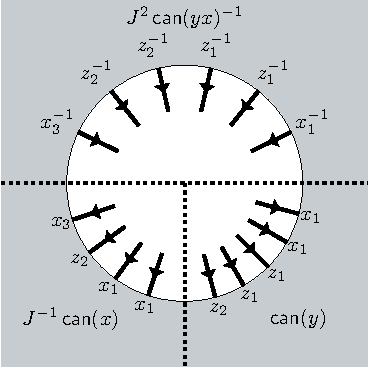
\includegraphics{MagicSquare-figure27.pdf}}
		    & $\longrightarrow$ &
			\resizebox{0.3\textwidth}{!}{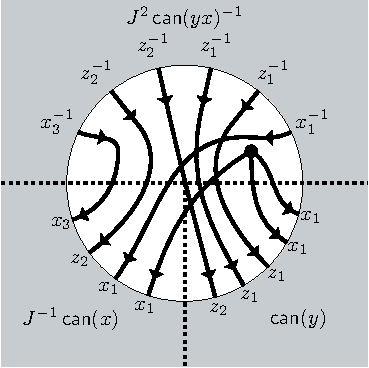
\includegraphics{MagicSquare-figure28.pdf}}
		    & $\longrightarrow$ &
			\resizebox{0.3\textwidth}{!}{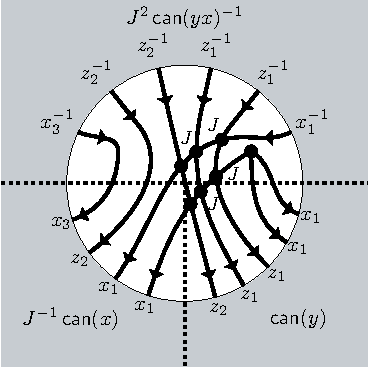
\includegraphics{MagicSquare-figure29.pdf}}
		\end{tabular}
	}
	\caption{Set $d = n = 3$ and $x = J\1x_1^2z_2x_3$, $y = x_1^2z_1^2z_2$. Then $\can(yx)\1 = J^{-2}x_3^{-1}z_2^{-2}z_1^{-2}x_1^{-1}$. The group picture witnesses that $J\1\can(x) J^2\can(yx)\1 \can(y) = J^4 = J$, from which it follows by scalar multiplication that $\can(x)\can(yx)\1\can(y) = 1$.}
	\label{fig:small-group-pictures-pauli-n}
\end{figure}


\subsection{Self-testing the Magic Square}
Recall the definition of the Magic Square game from Example \ref{example:magic-square}. 

\begin{definition}[Ideal strategy for Magic Square LCS game $\pmod 2$] 
	See Figure \ref{eq:mermin-peres-magic-square}. Let $A_e$ be the operator which appears on the right-hand side in the same spot as variable $e$ appears on the left-hand side. Set $A_e^{(v)}:= A_e$ for all $v$. Then set $B_e = \bar{A_e}$ (where any choice of basis works for the conjugation).  Set $\ket\psi = \ket{\text{EPR}}^{\otimes 2}$. We define $\{A_e^{(v)}\}, \{B_e \}, \ket\psi$ to be the \emph{ideal strategy} for the Magic Square game $\pmod 2$.
\end{definition}
Notice that the $B_e$ are defined only up to local isometry, because of the freedom in the choice of basis for conjugation.

\begin{figure}[!b]
	\begin{center}
	\begin{tabular}{m{0.4\textwidth}m{0.4\textwidth}}
		\resizebox{!}{0.22\textheight}{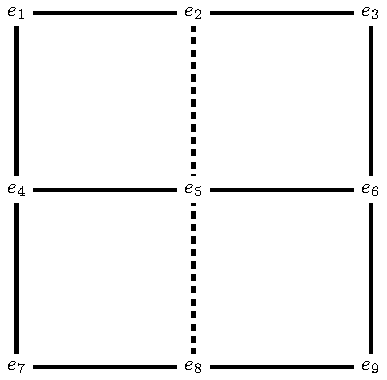
\includegraphics{MagicSquare-figure30.pdf}}
		&
		\resizebox{!}{0.22\textheight}{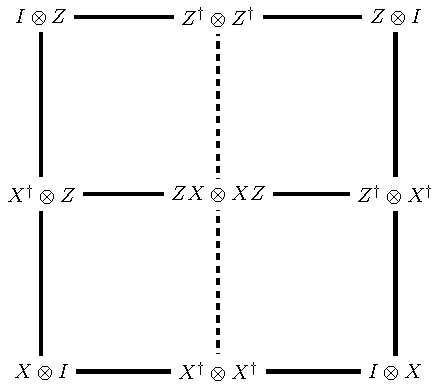
\includegraphics{MagicSquare-figure31.pdf}}
	\end{tabular}
	\end{center}
	\caption{The standard operator solution for the Magic Square.}
	\label{eq:mermin-peres-magic-square}
\end{figure}

The robust self-testing theorem for the Magic Square game is the following.
\begin{thm}\label{thm:robust-self-testing-square}
The Magic Square game mod $2$ self-tests the ideal strategy with perfect completeness and $O(\e)$-robustness.
\end{thm}
To prove this, we'll make a direct application of Theorem \ref{thm:robust-self-testing}. However, we'll use the tighter bounds stated in the appendix as Theorem \ref{thm:robust-self-testing-appendix}. We will check that all of its conditions are satisfied by a series of lemmas. 
Throughout, let $\G_2$ be the solution group for the Magic Square game over $\Z_2$. We'll start by identifying $\G_2$ as a group of Pauli operators.


\begin{prop}\label{prop:solution-group-square}
	$\G_2\cong \mathcal{P}_{2}^{\otimes 2}$.
\end{prop}

\begin{cor}\label{cor:G2-satisfies-conditions-4-5}
	$\G_2$ satisfies condition \eqref{assumption:group-test-appendix} of Theorem \ref{thm:robust-self-testing-appendix}. (This is the same as condition \eqref{assumption:w-p-irreps} of Theorem \ref{thm:robust-self-testing}.)
\end{cor}
\begin{proof}[Proof of corollary]
	Let $\tau = \tau_1^{(2)}$ as defined in Definition \ref{def:representations-pauli-group}. By Proposition \ref{prop:representations-pauli-group}, $\G_2$ group-tests $\tau$, giving \eqref{assumption:group-test-appendix}.
\end{proof}

We prove Proposition \ref{prop:solution-group-square} with two lemmas.

\begin{lemma}\label{lemma:commutator-subgroup-square}
	The commutator subgroup $[\G_2,\G_2]$ is $\Braket J$, 
	the cyclic subgroup generated by $J$.
\end{lemma}
\begin{proof}
	First, note that $J$ commutes with everything by construction.
	Next, see that each pair of generators of $\G_2$ has a commutator which is a power of $J$, and that $J$ commutes with all generators. If $w_1,w_2$ are words in the generators, then it holds by induction on the lengths of the words that $w_1w_2 = J^aw_2w_1$ for some $a\in \Z_2$. This proves the inclusion $\G_2' \seq \Braket J$. The reverse inclusion is immediate.
\end{proof}

\begin{lemma}\label{prop:four-edges}
	For generators $s_1,s_2 \in \G_2$, say that the pair $\pair{s_1}{s_2}$ is \emph{intersecting} if the corresponding edges in the constraint graph are incident on a common vertex.
 	Let $x_1,x_2,z_1,z_2$ be any generators of $\G_2$ such that $\set{x_1,x_2},\set{z_1,z_2},\set{x_1,z_2},\set{z_1,x_2}$ are interesecting pairs, while $\set{x_1,z_1},\set{x_2,z_2}$ are not.
 	Then
 	\begin{enumerate}
 		\item\label{item:prop-four-edges-1} $[x_1,z_1] = J = [x_2,z_2]$, and
 	 	\item\label{item:prop-four-edges-2} $\set{x_1,x_2,z_1,z_2, J}$ generates $\G_2$.
 	\end{enumerate}
 \end{lemma} 
 \begin{proof}

 	\ref{item:prop-four-edges-1}. If $x_1$ and $z_1$ are any pair of edges not sharing a vertex, then the group picture of Figure \ref{fig:k33-generators} establishes the twisted commutation relation. If $x_2$ and $z_2$ are any other pair of edges which do not share a vertex, then there is an automorphism of the graph $K_{3,3}$ sending $x_1\mapsto x_2$ and $z_1\mapsto z_2$. Therefore, we can draw the same group picture with a different labeling to prove that $x_2$ and $z_2$ share the same twisted commutation relation.
 	
 	\ref{item:prop-four-edges-2}. See Figure \ref{fig:k33-generators}. Suppose some vertex has only one black edge. Then the group element labeling the black edge is equal to some product of $J$ and the group elements labeling the blue edges at that vertex. So the group generated by the blue edges and $J$ contains the black edge. By the sequence of pictures in Figure \ref{fig:k33-generators}, we see that the four blue edges, together with $J$, generate all nine of the edges. Therefore, they generate all of $\G_2$.
 \end{proof}
From here on, we fix the identification $x_1 = e_7, x_2 = e_9, z_1 = e_3, z_2 = e_1$ (c.f.\ Figure \ref{eq:mermin-peres-magic-square}).

\begin{proof}[Proof of Proposition \ref{prop:solution-group-square}]
	We have the same set of generators for both groups. This gives a surjective function $\mathcal{P}_2^{\otimes 2}\to \G_2$. We've seen that the generators of $\G_2$ satisfy the relations defining $\mathcal{P}_2^{\otimes 2}$; this implies that the function is a group homomorphism. All that remains to check is that the map is injective, i.e.\ has trivial kernel. This holds if the relations of $\G_2$ hold for the preimages of the $e_i$ in $\mathcal{P}_2^{\otimes 2}$. This follows from the fact that the square of operators \eqref{eq:mermin-peres-magic-square} is a Mermin--Peres magic square in the usual sense, i.e.\ operators in the same row or column commute, the products across each row and down the first two columns are $I$, and the product down the last column is $-I$. *Notice that this step fails for the Magic Square game mod $d \neq 2$.*
	
\end{proof}

\begin{figure}[!b]
	\begin{tabular}{m{0.3\textwidth}m{0.05\textwidth}m{0.3\textwidth}m{0.05\textwidth}m{0.3\textwidth}}
	\resizebox{0.3\textwidth}{!}{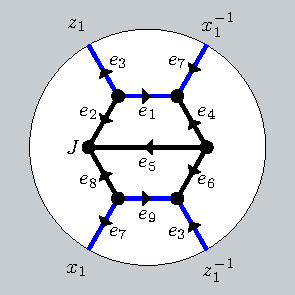
\includegraphics{MagicSquare-figure32.pdf}}
        &$\longrightarrow$
	&\resizebox{0.3\textwidth}{!}{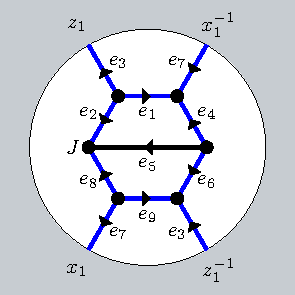
\includegraphics{MagicSquare-figure33.pdf}}
        &$\longrightarrow$
	&\resizebox{0.3\textwidth}{!}{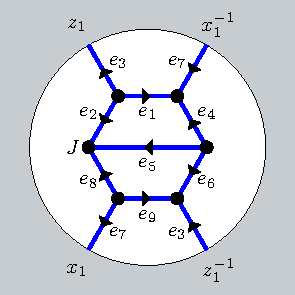
\includegraphics{MagicSquare-figure34.pdf}}
	\end{tabular}

    \caption{The group picture proves that $x_1z_1x_1\1z_1\1 = J$ in the solution group for the magic square with the identification $x_1 = e_7, x_2 = e_9, z_1 = e_3, z_2 = e_1$. (Compare Figure \ref{eq:mermin-peres-magic-square}.) The blue-colored edges illustrate that $\set{x_1, z_1, x_2, z_2, J}$ generates the solution group for the magic square.}
    \label{fig:k33-generators}
\end{figure}

\begin{lemma}\label{lemma:small-group-pictures-square}
	Suppose $\m P$ is a $\mathcal{P}_2^{\otimes 2}$-picture in which each generator and relation appears at most $m$ times. Then there is a $\G_2$-picture $\m P'$ witnessing the same equation in which each generator and relation appears at most $3m$ times.
\end{lemma}
This allows us to control the size of group pictures for any relation in $\G_2$ which uses only the letters $x_1,x_2,z_1,z_2,J$. For relations using the other generators, we'll use Lemma \ref{lemma:G2-m0-equals-1}
\begin{proof}
	The generators labeling $\m P$ can be reinterpreted as generators of $\G_2$. $\m P$ has at most $2m$ twisted commutation relations, and the rest of the relations are already relations of $\G_2$. Form $\m P'$ by replacing each twisted commutation relation with a $\G_2$-group picture of the form of Figure \ref{fig:k33-generators}. Each subpicture replacement adds at most one use of each generator and relation.
\end{proof}

\begin{figure}
	\caption{
	The left-hand picture proves that $e_6(x_2z_1) = 1$. This is equivalent to proving $e_6 = \can(e_6) = z_1\1x_2\1$.
	}
	\label{fig:G2-m0-equals-1}
	\begin{center}
	\begin{tabular}{m{0.3\textwidth}m{0.3\textwidth}m{0.3\textwidth}}	
		\resizebox{0.3\textwidth}{!}{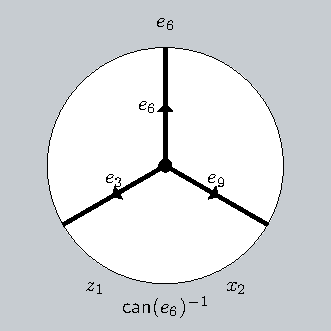
\includegraphics{MagicSquare-figure35.pdf}}
		&
		&\resizebox{0.3\textwidth}{!}{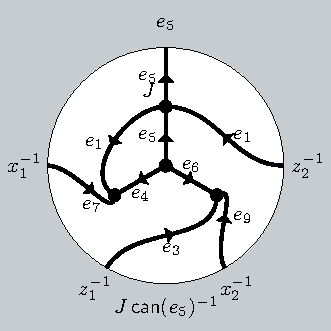
\includegraphics{MagicSquare-figure36.pdf}}
	\end{tabular}
	\end{center}
	\caption{
	The right-hand picture proves that $e_5(x_1z_1x_2z_2)\1 = J$. Multiplying both sides by $J\1$, we see that this is equivalent to proving $e_5 = \can(e_5) = Jx_1z_1x_2z_2$. The picture has been drawn with a twisted commutation relation between $e_1$ and $e_5$. To get a valid $\G_2$-picture, this relation must be expanded to a subpicture of the form of Figure \ref{fig:k33-generators}, just as in the proof of Lemma \ref{lemma:small-group-pictures-square}. 
	The new picture thus formed uses each generator and relation at most $3$ times.
	}
	\label{fig:G2-m0-equals-1-b}
\end{figure}

Let $\can$ be the canonical form from \ref{lemma:canonical-form} composed with the isomorphism $\G_2 \cong \mathcal{P}_2^{\otimes 2}$.
\begin{lemma}\label{lemma:G2-m0-equals-1}
	For each generator $e\in E$, the equation $\can(e)e\1 = 1$ has a group picture in which each generator and relation appear at most $3$ times. 
\end{lemma}
\begin{proof}

	Either $\can(e) = e$ as words already, or there is a picture similar to one of the pictures in Figures \ref{fig:G2-m0-equals-1},\ref{fig:G2-m0-equals-1-b}. (Here by ``similar'' we mean ``identical up to relabeling of edges''.) 
\end{proof}


\begin{proof}[Proof of Theorem \ref{thm:robust-self-testing-square}]
We want to apply Theorem \ref{thm:robust-self-testing-appendix}, so we check each of its conditions. The magic square has at most $3$ variables in each equation, so we can take $l_0 = 3$ in condition \eqref{assumption:bounded-degree-appendix}. By Lemma \ref{lemma:G2-m0-equals-1}, we can take $m_0 = 3$ in condition \eqref{assumption:small-pictures-appendix}. By Lemmas \ref{lemma:small-group-pictures-square} and \ref{lemma:small-group-pictures-pauli-n}, we can take $m = 108\cdot 2^2$  in condition \eqref{assumption:small-pictures-w-appendix}. The final two conditions were shown to hold in Corollary \ref{cor:G2-satisfies-conditions-4-5}. We hence apply Theorem \ref{thm:robust-self-testing-appendix} to get the desired conclusion.
\end{proof}

\subsection{Self-testing the Magic Pentagram}
Recall the definition of the Magic Pentagram game from Example \ref{example:magic-pentagram}. 

\begin{definition}[Ideal strategy for Magic pentagram $\pmod 2$] 
	In Figure \ref{fig:magic-pentagram}, associate each operator in the left-hand pentagram with the corresponding variable in the right-hand pentagram. Set $A_e^{(v)}$ to the operator corresponding to $e$, and denote the latter by $A_e$, so that we have $A_e^{(v)} = A_e$ for all $v$. Then set $B_e = \bar{A_e}$ (where any choice of basis works for the conjugation). 
\begin{figure}[h]
	\begin{tabular}{m{0.4\textwidth}m{0.1\textwidth}m{0.4\textwidth}}
		\resizebox{0.4\textwidth}{!}{
			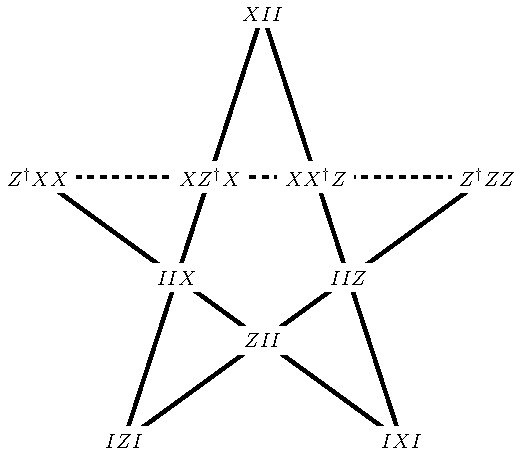
\includegraphics{MagicSquare-figure37.pdf}
	   	}
	   	&&
		\resizebox{0.4\textwidth}{!}{
			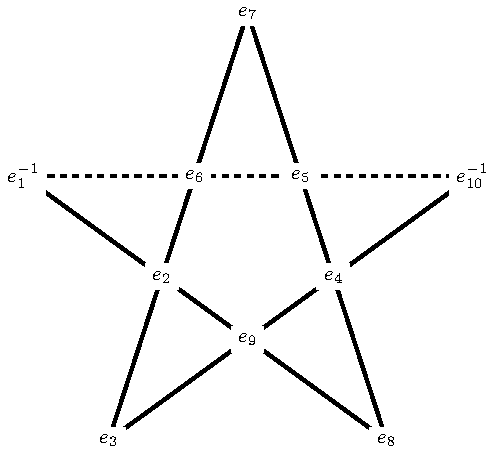
\includegraphics{MagicSquare-figure38.pdf}
	   	}
	\end{tabular}
	\caption{The standard operator solution for the Magic Pentagram.}
	\label{fig:magic-pentagram}
\end{figure}

	Set $\ket\psi = \ket{\text{EPR}_2}^{\otimes 3}$. We define $\{A_e^{(v)}\}, \{B_e \}, \ket\psi$ to be the \emph{ideal strategy} for the Magic Pentagram game.
\end{definition}

The robust self-testing theorem for the Magic Pentagram game is the following.
\begin{thm}\label{thm:robust-self-testing-pentagram}
The Magic Pentagram game mod $2$ self-tests the ideal strategy with perfect completeness and $O(\e)$-robustness.
\end{thm}
Again, to prove this, we will make a direct application of Theorem \ref{thm:robust-self-testing}, but we will use the tighter bounds stated in the appendix as Theorem \ref{thm:robust-self-testing-appendix}.



Let $\G_3$ be the solution group for the Magic Pentagram. We give the proof details only where they differ from the Magic Square case. 


\begin{prop}\label{prop:solution-group-pentagram}
	$\G_3\cong \mathcal{P}_2^{\otimes 3}$. 
\end{prop}
\begin{cor}\label{cor:G3-satisfies-conditions-4-5}
	$\G_2$ satisfies condition \eqref{assumption:group-test-appendix} of Theorem \ref{thm:robust-self-testing-appendix} with $\tau = \tau_1^{(3)}$ from Definition \ref{def:representations-pauli-group}.
\end{cor}


\begin{lemma}\label{lemma:commutator-subgroup-pentagram}
	The commutator subgroup $[\G_3,\G_3]$ is $\Braket J$, 
	the cyclic subgroup generated by $J$.
\end{lemma}

\begin{lemma}\label{prop:six-edges}
 	Let $x_1,x_2,x_3,z_1,z_2,z_3$ be any generators of $\G_3$ such that in the linear constraint graph, the edge pairs $\set{x_i,x_j},\set{z_i,z_j},\set{x_i,z_j},i\neq j$ are \emph{intersecting} (see Lemma \ref{prop:four-edges}), while the edge pairs $\set{x_i,z_i}$ are not. 
 	Then
 	\begin{enumerate}
 		\item\label{item:prop-six-edges-1} $[x_i,z_i] = J $, and
 	 	\item\label{item:prop-six-edges-2} $\set{x_i,z_i, J\;i\leq 3}$ generates $\G_3$.
 	\end{enumerate}
 \end{lemma} 
 \begin{proof}

 	\ref{item:prop-six-edges-1}.
 	If $x_1$ and $z_1$ are any pair of edges not sharing a vertex, then the group picture of Figure \ref{fig:k5-generators} establishes the twisted commutation relation. If $x_i$ and $z_i$ are any other pair of edges which do not share a vertex, then there is an automorphism of the graph $K_{5}$ sending $x_1\mapsto x_i$ and $z_1\mapsto z_i$. Therefore, we can draw the same group picture with a different labeling to prove that $x_i$ and $z_i$ share the same twisted commutation relation.
 	
 	\ref{item:prop-six-edges-2}.
 	See Figure \ref{fig:k5-generators}, which is interpreted the same way as Figure \ref{fig:k33-generators} from the Magic Square case.
 \end{proof}
We fix the identification $x_1 = e_7, z_1 = e_9, x_2 = e_8, z_2 = e_3, x_3 = e_2, z_3 = e_4$ (c.f.\ Figure \ref{fig:magic-pentagram}.)

\begin{figure}
    \caption{
    The leftmost group picture proves that $x_1z_1x_1\1z_1\1 = J$ in $\G_3$, with $x_1 = e_7, z_1 = e_9$. Identifying further $x_2 = e_8, z_2 = e_3, x_3 = e_2, z_3 = e_4$ and following the color of the edges shows that $\set{x_i,z_i, J\;i\leq 3}$ generates $\G_3$.
    }
    \label{fig:k5-generators}
	\begin{center}
	\begin{tabular}{
	m{0.3\textwidth}
	m{0.03\textwidth}
	m{0.3\textwidth}
	m{0.3\textwidth}
	}
		\resizebox{0.3\textwidth}{!}{
			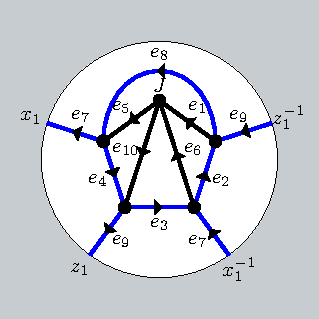
\includegraphics{MagicSquare-figure39.pdf}
	    	}
	     &$\longrightarrow$
	 	 &\resizebox{0.3\textwidth}{!}{
			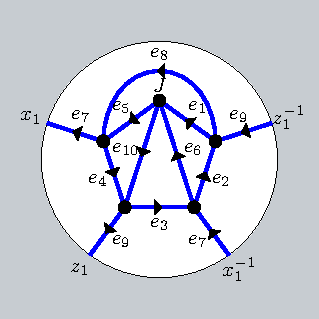
\includegraphics{MagicSquare-figure40.pdf}
	        }
		& \resizebox{0.3\textwidth}{!}{
			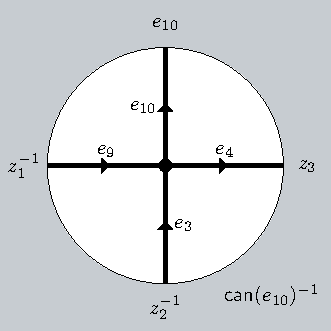
\includegraphics{MagicSquare-figure41.pdf}
	        }
	\end{tabular}
	\end{center}
	\caption{
		The rightmost figure is a $\G_3$-picture showing $\can(e_{10}) = z_1z_2z_3\1$.
	}
	\label{fig:G3-m0-equals-1}
\end{figure}


\begin{proof}[Proof of Proposition \ref{prop:solution-group-pentagram}]
	As in the Magic Square case, all that remains to check is that the generators of $\mathcal{P}_2^{\otimes 3}$ satisfy the relations of $\G_3$. This amounts to checking that the pentagram of operators in Figure \ref{fig:magic-pentagram} is a $2$-dimensional Mermin Magic Pentagram in the usual sense, i.e.\ operators on the same line commute, the alternating products across the four solid lines are each $I$, and the alternating product across the dashed line is $-I$.
\end{proof}

\begin{lemma}\label{lemma:small-group-pictures-pentagram}
	Suppose $\m P$ is a $\mathcal{P}_2^{\otimes 3}$-picture in which each generator and each relation appears at most $m$ times. Then there is a $\G_3$-picture $\m P'$ witnessing the same equation in which each generator and each relation appears at most $4m$ times.
\end{lemma}
\begin{proof}
	We use the same proof as in the Magic Square case, but now there are up to $3m$ twisted commutation relations in $\m P$.
\end{proof}

Let $\can$ be the canonical form from Lemma \ref{lemma:canonical-form} composed with the isomorphism $\G_3 \cong \mathcal{P}_2^{\otimes 3}$.
\begin{lemma}\label{lemma:G3-m0-equals-1}
	For each generator $e\in E$, the equation $\can(e)e\1 = 1$ has a group picture in which each generator and relation appear at most once. 
\end{lemma}
\begin{proof}

	Either $\can(e) = e$ as words already, or there is a picture similar to the picture in Figure \ref{fig:G3-m0-equals-1}.
\end{proof}

\begin{proof}[Proof of Theorem \ref{thm:robust-self-testing-pentagram}]
Again we wish to apply Theorem \ref{thm:robust-self-testing-appendix}, so we check each of its conditions. The Magic Pentagram constraint system has at most $4$ variables in each equation, so we can take $l_0 = 4$. Let $\can$ be the canonical form for $\mathcal{P}_2^{\otimes 3}$ from Lemma \ref{lemma:canonical-form} composed with the group isomorphism $\mathcal{P}_2^{\otimes 3} \cong \G_3$. By Lemma \ref{lemma:G3-m0-equals-1}, we can take $m_0 = 1$. By Lemmas \ref{lemma:small-group-pictures-square} and \ref{lemma:small-group-pictures-pauli-n}, we can take $m = 162\cdot 2^2$. That the final two conditions are satisfied is Corollary \ref{cor:G3-satisfies-conditions-4-5}. Applying Theorem \ref{thm:robust-self-testing-appendix} gives the desired statement.
\end{proof}


\subsection{Self-testing $n$ pairs of maximally entangled qubits and $n$-qubit Paulis}

Self-testing in parallel has gained recent interest both as a potential tool in cryptographic protocols, and as a simple way to witness high-dimensionality of a quantum system. Various recent results have shown self-testing of $n$ maximally entangled pairs of qubits, and associated $n$-qubit Pauli measurements, in particular using copies of the Magic Square game \cite{coladan17, CN16}. In this section, we show how our general self-testing result of Theorem \ref{thm:robust-self-testing} allows to produce a similar result.

We will introduce first a notion of product of LCS games. Informally, we form the product of LCS games by adding new equations to enforce commutativity between each variable in one game with each variable in the others. 
The main motivation for this definition is that we can express the solution group of the product as an appropriate product of the solution groups. First, we introduce our notion of product for groups over $\Z_d$ (we will only make use of it mod $2$ though).

\begin{definition}
	Let $G_i = \braket{S_i:R_i}_{\Z_d}$ be a family of groups presented over $\Z_d$. Define their \emph{product over $\Z_d$} as
	\begin{align}
		\prod^{\Z_d}_i G_i :=
		\Braket{
		\bigsqcup_i S_i:
		\bigsqcup_i R_i \sqcup R_\text{prod}
		}_{\Z_d},
		&&
		R_\text{prod} = \set{[s,s']\;s\in S_i, s'\in S_j, i\neq j}.
	\end{align}
	Here the symbol $\sqcup$ denotes the disjoint union.
\end{definition}
One can check that this product is the categorical product in the category which has objects the groups presented over $\Z_d$ and has maps the group homomorphisms that send $J\mapsto J$. Therefore it obeys the usual properties one expects from a product. In particular it has an equivalent definition as a repeated application of an associative binary product $\overset{\Z_d}\times$. The following is easy to check from Definition \ref{definition:n-qudit-pauli-group}.

\begin{lemma}
	The $n$-qudit Pauli group is the $n$-fold product over $\Z_d$ of the $1$-qudit Pauli group, i.e.\
	\begin{equation}
		\m P_d^{\otimes n} = \prod^{\Z_d}_{i\in[n]}\m P_d^{\otimes 1}.
	\end{equation}
	 As a corollary, 
	 $\m P_d^{\otimes n_1} \overset{\Z_d}\times \m P_d^{\otimes n_2} = \m P_d^{\otimes(n_1+n_2)}$.
\end{lemma}


\begin{definition}[LCS game product]
\label{def:lcs-game-product}
	Let $G_i=\LCS(\mathbf H_i, l_i, \Z_d)$, $i\in [n]$ be LCS games over $\Z_d$ with $\mathbf H_i=(H_i,V_i,E_i)$. We define their \emph{product LCS game} as $\prod_iG_i:= \LCS(\mathbf H, l, \Z_d)$, where $\mathbf H = (H,V,E)$ andbbb
	\begin{align}
	V &= \left(\bigsqcup_i V_i\right)\sqcup V_\text{prod}
	&V_\text{prod} &= \set{v_{xy}\; x\in E_i, y\in E_j, i\neq j}
	\\E &= \left(\bigsqcup_i E_i\right)\sqcup E_\text{prod}
	&E_\text{prod} &= \set{e_{xy}\; x\in E_i, y\in E_j, i\neq j}
	\end{align}
	In words, we add one equation and one variable for each pair of variables $x,y$ living in distinct factor games. We call the new variable $e_{xy}$, and the equation is
	\begin{equation}
		x + y - e_{xy} = 0.
	\end{equation}
	The definition of the equations can be formalized as follows.
	\begin{align}
	l(v) &= \begin{cases}
		l_i(v), &\text{ if }v\in V_i\\
		0, 		&\text{ if }v\in V_\text{prod}\\
		\end{cases}
	&
	H(v,e) &= \begin{cases}
		H_i(v,e), &\text{ if }v \in V_i\text{ and }e\in E_i\\
		1, &\text{ if }v = v_{xy}\text{ and }e \in \pair xy\\
		-1, &\text{ if }v = v_{xy}\text{ and }e = e_{xy}\\
		0, &\text{ otherwise }
		\end{cases}
	\end{align}
\end{definition}

\begin{lemma}
\label{lemma:lcs-game-product}
Let $G_0 = \prod_{i=1}^nG_i = \LCS(\mathbf H_0, l_0, \Z_d)$.
~\begin{enumerate}
	\item If each of the $G_i$ satisfy 
	$\forall v:\sum_e\abs{H_i(v,e)} \leq \Delta_i$ then $G_0$ satisfies the same with
	$\Delta_0 = \max\left(\set{\Delta_i}\cup\set{3}\right)$.
	\item $\abs{E_0} \leq (\sum_i\abs{E_i})^2$
	\item $\abs{V_0} = \abs {E_0} + \sum_i \abs {V_i}$
	\item\label{item:LCS-product-is-functorial} Let $\G_i = \G(\mathbf H_i,l_i,\Z_d)$. Then $\G_0 = \prod\limits^{\Z_d}_{i>0}\G_i$. 
\end{enumerate}
\end{lemma}
\begin{proof}
	We prove only \eqref{item:LCS-product-is-functorial}, which is less straightforward than the rest.

	Let $\G = \prod\limits_{i>0}^{\Z_d}\G_i$. There's a clear inclusion map $\iota:\G\into \G_0$, since the generators of the former are a subset of the generators of the latter.  To see that $\iota$ is a homomorphism, we show that the relations of $\G$ are a subset of the relations of $\G_0$. For each commutation relation introduced by the group product, there is an equation in the product containing the same variables. So the solution group $\G_0$ has a corresponding commutation relation.
	To see that this map is surjective, notice that $e_{xy} = xy$ in $\G_0$, so all of the generators of $\G_0$ lie in the image of $\iota$. To see that $\iota$ is injective, check that every relation in the presentation $\G_0$ is already true of the pre-image elements in $\G$. 
\end{proof}

\begin{definition}
	Let $G_2$ and $G_3$ be the Magic Square and Magic Pentagram LCS games over $\Z_2$, respectively.
	For $n\geq 4$, construct $G_n$ as an LCS game product as follows:
	\begin{align}
		G_{2k} := \prod_{i\in [k]}G_2,
		&&
		G_{2k+1} :=\prod(\underbrace{G_2,\ldots, G_2}_{k-1}, G_3),
	\end{align}
	where $\prod$ is the LCS game product from Definition \ref{def:lcs-game-product}. 
\end{definition}
From Lemma \ref{lemma:lcs-game-product} and properties of $G_2$ and $G_3$, we can deduce basic properties of $G_n$.
\begin{lemma}~
\label{lemma:basic-Gn-properties}
	\begin{enumerate}
		\item $G_n$ satisfies $\forall v:\sum_e \abs{H_n(v,e)} \leq 4$.
		\item $\abs{E_n} \leq \abs{V_n} \leq 25n^2$.
		\item $G_n$ has solution group $\G_n \cong \m P_2^{\otimes n}$
	\end{enumerate}
\end{lemma}

Next, we describe the winning strategy for the game $G_n$. First, we give an abstract description, and then we unpack it into a concrete description. Understanding either description should suffice to appreciate Theorem \ref{thm:self-testing-pauli-LCS}.

\begin{definition}[Ideal strategy for the game $G_n$, abstract]
	Let $\tau_n^{(1)}: \mathcal{P}_2^{\otimes n}\to U(\C^2)^{\otimes n}$ be as in Definition \ref{def:representations-pauli-group}. Then let $\tau$ be composition of that map with the isomorphism $\mathcal{P}_2^{\otimes n}\cong \G_n$. The ideal strategy is that which follows from applying the construction of Proposition \ref{prop: perfect strategy} to the operator solution $\tau$.
\end{definition}

As a structural hint for what follows, notice that each observable measured by the provers is a Pauli operator of weight at most $5$. (It is either a magic square operator, a magic pentagram operator, a tensor product of magic square operators, or a tensor product of a Magic Square operator with a Magic Pentagram operator.) 

Recall by the definition of product game, that, for $n = 2k$, $V_n = \bigsqcup_{i \in [k]} V_2^{(i)} \sqcup V_\text{prod}$ and $E_n = \bigsqcup_{i \in [k]} E_2^{(i)} \sqcup E_\text{prod}$ where $V_2^{(i)}$ and $E_2^{(i)}$ are the vertex and edge sets for the $i$th copy of the magic square game, and $V_\text{prod} = \set{v_{xy}, x\in E_i, y\in E_j, i\neq j}$ and $E_\text{prod} = \set{e_{xy}, x\in E_i, y\in E_j, i\neq j}$. Similarly, for $n=2k+1$, $V_n = \bigsqcup_{i \in [k-1]} V_2^{(i)} \sqcup V_3 \sqcup V_\text{prod}$ and $E_n = \bigsqcup_{i \in [k-1]} E_2^{(i)} \sqcup E_3 \sqcup V_\text{prod}$ where $V_3$ and $E_3$ are the vertex and edge sets corresponding to the magic pentagram game. 

\begin{definition}[Ideal strategy for the game $G_n$]
Let $\{A^{\text{sq}}_e\}$, $\{B^{\text{sq}}_e\}$ and $\{A^{\text{pt}}_e\}$, $\{B^{\text{pt}}_e\}$  be observables from the ideal strategies of the magic square and magic pentagram games mod $d$ respectively.
\begin{itemize}
\item For $n = 2k$, the $A_e^{(v)}$ are observables on $\C^{2^n}$ (which we think of as $k$ copies of $\C^{2^2}$). If $v \in V_2^{(i)}$ and $e \in E_2^{(i)}$, let $A_e^{(v)} = (A^{\text{sq}}_e)_i \otimes I := A_e$, where the subscript indicates that the observable acts on the $i$th of the $k$ copies, and the identity is on everything else; if $v = v_{ey}$ or $v = v_{xe} \in V_\text{prod}$ and $e \in E_2^{(i)}$, let $A_e^{(v)} =  (A^{\text{sq}}_e)_i \otimes I := A_e$; if $v = v_{xy} \in V_\text{prod}$ and $e = e_{xy}$ for $x \in E_2^{(i)}$ and $y \in E_2^{(j)}$, then let $A_e^{(v)}$ = $(A^{\text{sq}}_x)_i \otimes (A^{\text{sq}}_y)_j \otimes I := A_e$. Finally, let $B_e = \bar{A_e}$.
\item For $n = 2k+1$, the observables are on $\C^{2^n}$ (which we think of as $k-1$ copies of $\C^{2^2}$ and one copy of $\C^{2^3}$). The only changes from the even case are the following: if $v \in V_3$ and $e \in E_3$, let $A_e^{(v)} = (A^{\text{pt}}_e)_k \otimes I := A_e$, where the $k$ subscript denotes the last $\C^3$ register; if $v = v_{ey}$ or $v = v_{xe} \in V_\text{prod}$ and $e \in E_3^{(i)}$, let $A_e^{(v)} =  (A^{\text{pt}}_e)_k \otimes I := A_e$; if $v = v_{xy} \in V_\text{prod}$ and $e = e_{xy}$ for $x \in E_2^{(i)}$ and $y \in E_3$, then let $A_e^{(v)}$ = $(A^{\text{sq}}_x)_i \otimes (A^{\text{pt}})_k \otimes I := A_e$, and similarly for the symmetric case. As before, let $B_e = \bar{A_e}$.
%if $v \in V_2^{(i)}$ and $e \in E_2^{(i)}$, let $A_e^{(v)}$ let $A_e^{(v)} = (A^{\text{sq}}_e)_i \otimes I := A_e$; if $v \in V_3$ and $e \in E_3$, let $A_e^{(v)} = (A^{\text{pt}}_e)_k \otimes I := A_e$, where the $k$ subscript denotes the last $\mathbb{C}^3$ register; if $v = v_ey$ or $v = v_xe \in V_\text{prod}$ and $e \in E_2^{(i)}$, let $A_e^{(v)} =  (A^{\text{sq}}_e)_i \otimes I := A_e$; if $v = v_ey$ or $v = v_xe \in V_\text{prod}$ and $e \in E_3^{(i)}$, let $A_e^{(v)} =  (A^{\text{pt}}_e)_k \otimes I := A_e$; if $v = v_{xy} \in V_\text{prod}$ and $e = e_{xy}$ for $x \in E_2^{(i)}$ and $y \in E_2^{(j)}$, then let $A_e^{(v)}$ = $(A^{\text{sq}}_x) \otimes A^{\text{sq}}_y \otimes I := A_e$; if $v = v_{xy} \in V_\text{prod}$ and $e = e_{xy}$ for $x \in E_2^{(i)}$ and $y \in E_3$, then let $A_e^{(v)}$ = $(A^{\text{sq}}_x))i \otimes (A^{\text{pt}})_k \otimes I := A_e$. Finally, let $B_e = \bar{A_e}$.
\end{itemize}
Set $\ket\psi = \ket{\text{EPR}_2}^{\otimes n}$. Define $\set{A_e^{(v)}}$, $\set{B_e}$, $\ket\psi$ to be the ideal strategy.
\end{definition}


\begin{thm}\label{thm:self-testing-pauli-LCS}

The product game $G_n$ mod $2$ self-tests the ideal strategy with perfect completeness and $O(n^{10}\e)$-robustness.
\end{thm}

\begin{lemma}\label{lemma:small-group-pictures-pauli-LCS}
	Suppose $\m P$ is a $\mathcal{P}_2^{\otimes n}$-picture in which each relation and each generator appears at most $m$ times. Then there is a $\G_n$-picture $\m P'$ witnessing the same equation in which each relation and each generator appears at most $4m$ times. 
\end{lemma}
\begin{proof}
	As in Lemmas \ref{lemma:small-group-pictures-square} and \ref{lemma:small-group-pictures-pentagram}, we take $\m P$ and replace the twisted commutation relations with small subpictures. There are at most $3m$ twisted commutation relations from each factor game $G_2$ or $G_3$, and each one is replaced by a $\G_2$- or $\G_3$-picture. Each of these replacements adds at most one instance of each generator and relation.
\end{proof}

Let $\can$ be the canonical form from \ref{lemma:canonical-form} composed with the isomorphism $\G_n \cong \mathcal{P}_2^{\otimes n}$.
\begin{lemma}
\label{lemma:small-group-pictures-w-pauli-LCS}
	For each generator $e\in E_n$, the equation $\can(e)e\1 = 1$ has a group picture in which each generator and relation appear at most three times. 
\end{lemma}
\begin{proof}
	If $e$ comes from a Magic Square factor or a Magic Pentagram factor, then we apply Lemma \ref{lemma:G2-m0-equals-1} or \ref{lemma:G3-m0-equals-1}, respectively. If $e = e_{xy}$ is an auxiliary variable, then we glue the pictures for $x$ and $y$ together.
\end{proof}



\begin{proof}[Proof of Theorem \ref{thm:self-testing-pauli-LCS}]
	We again seek to apply theorem \ref{thm:robust-self-testing-appendix}, so we check each of its conditions. From Lemma \ref{lemma:basic-Gn-properties}, we have 
	$l_0 = 4$. 
	From Lemma \ref{lemma:small-group-pictures-w-pauli-LCS}, we have $m_0 = 3$.  
	From Lemmas \ref{lemma:small-group-pictures-pauli-n} and \ref{lemma:small-group-pictures-pauli-LCS}, we have $m = 72\cdot 2^2n$.
	Finally, it follows from item $3$ of Proposition \ref{lemma:basic-Gn-properties} that $\G_n$ group-tests $\tau_1^{(n)}$, whose image contains an isomorphic copy of $\mathcal{P}_2^{\otimes n}$.  Then, applying Theorem \ref{thm:robust-self-testing-appendix} gives the desired bound.
	
\end{proof}


